\section{Joule-Thomson porous plug experiment}
	The Joule-Thomson porous plug experiment investigates how the temperature of a real gas changes when it expands through a porous barrier without performing external work. This setup models throttling processes used in refrigeration cycles. The experiment provides direct insight into the internal energy changes associated with real gas expansion. The observed temperature changes help define the Joule-Thomson coefficient.
	\begin{figure}[h!]
		\centering
		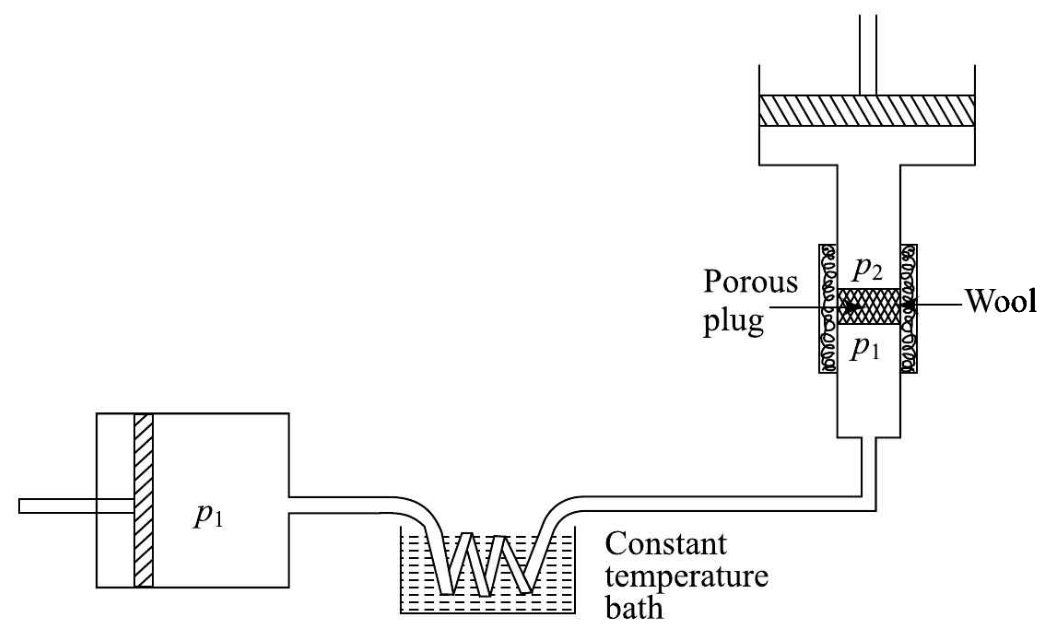
\includegraphics[width=0.6\textwidth]{figures/fig_porous-plug.png}
	\end{figure}
	
	In this experimental setup, a highly compressed gas is continuously forced at constant pressure to expand adiabatically and irreversibly through a porous plug kept in a non-conducting cylinder (as shown in the figure). The plug consists of a porous material, say cotton, wool, silk etc., and has a number of fine holes. Thus, a porous plus is equivalento a number of narrow orifices held in parallel.
	
	The gas flows from a high-pressure region to a low-pressure region through a porous plug. Since the process is adiabatic and no external work is done, the enthalpy remains constant, i.e.
	\begin{align*}
		H_1=H_2
	\end{align*}
	This is known as \textit{isenthalpic expansion}.
	
	\subsection{Joule-Thomson effect}
		The Joule-Thomson effect describes the temperature change experienced by a real gas during throttling at constant enthalpy. Depending on the nature of intermolecular forces, the gas may cool or warm upon expansion. The sign and magnitude of this effect are characterised by the Joule-Thomson coefficient. This behaviour is essential in refrigeration and liquefaction processes.
		
		The Joule-Thomson coefficient is:
		\begin{align*}
			\Aboxed{\mu_\text{JT}&=\qty(\pdv{T}{P})_H}
		\end{align*}
		\begin{itemize}
			\item If $\mu_\text{JT}>0$, the gas cools on expansion
			\item If $\mu_\text{JT}<0$, the warms up on expansion
		\end{itemize}
		
		The temperature at which $\mu_\text{JT}=0$ is known as the \textit{inversion temperature}, above which expansion causes heating and below which cooling occurs.